\section{Background}
\subsection{A Preface on Humanity and the Climate}
\begin{flushleft}\emph{
The development of humanity is not unlike the chirography of an Aristotelian tragedy. It starts with a simple/primitive species cradling a noble cause - to improve their chances of survival. Here the protagonist (humankind) develops a fatal flaw: an insecurity and latent distruction of their home due to a sudden rise to power.
Having acknowleged this flaw, we now strive to imporve our understanding of the universe, correct past mistakes and stem the tide of inevitable change. \vspace{\baselineskip}\linebreak
With tragedy being an imitation not of humanity, but of action and life, happiness and misery, it is only expected that such a comparison to our current affairs should stir feelings of catharsis when exploring our need for research and scientific advancement.
It is with that I begin this thesis with the begining of the planet, its atmosphere and consequently the start of humankind.
}
\end{flushleft}

% \section{Whence}
% This section describes the intial formation of an atmosphere, how this led to life, and ultimately the human race.
\subsection{Formation of the Atmosphere}
 ~4.5 billion years ago the Earth began as a disk of dust and gas orbiting our sun. The movement of such gasses produces a resonant drag instability, which causes them to clump together \citep{drag,planet}. As these `clumps' become denser, other forces come in to play and further increase their size. These eventually produced the hot mix of gas and solid which was to become Earth.
 As the Earth cooled, the vollotile componenets of the primodial gas cloud surrounding it begin to form an atmosphere. %Volcanic erruptions (outgassing) from the Earth's sruface
At this point in time oxygen was not only absent in the atmopshere, but also had many sinks within the Earths anoxidised crust. It was not until oxygenic photosynthesis (\citep{oxygenicphotosynthesis}) that the concentrations of oxygen in the atmosphere started to increase. Eventually the development of multicellular cyanobacteria\footnote{The phylum of phtosynthetic prokaryotic (cells not containing a distinct nucleus) bacteria - e.g. blue-green algae} resulted in biologically induced oxygen accumelating in the atmosphere, \citep{multicellular}. This led to the most significant climate event in the planets history: the Great Oxigenation Event (2.5 billion years ago), \citep{oxidation}. This increase of oxygen allowed oragnisms to become larger and more active, eventually resulting in the human race.
\subsection{Rise of the Homo Spiens (`Wise Man')}
About x million years ago there were many varieties of the homo genus. With the development of the human brain, energy transfer changed. A larger brain required more fuel, and therefore with the development of cooking\footnote{The first known case of indoor air pollution} humans were able to increase their...
This form on ingenuity eventually resulted in the ... industrial revolution.
This led to the first know source of indoor air pollution.
Ever since we have experienced issues regarding to this...

As part of this air pollution and climate have always been a concern for the human race. Concerns about lead in the air can be documented back as far as 6000 years ago [se ref, ], in ancient Rome [1145] and in 1285 where after a visit from Queen of England to a coal burning to Nottingham, the first air pollution act was deployed [1147].
air pollution = animals
air qulaity pollicy
kingxx
With the this increased capability, a language capable of communicating information, allowing for the ability to not only hunt larger prey but also.
Ability to metaphorical, allowed fruther knwoplege transfer , cvave paings and metaphoirical for people over 150 ....
REFERENCES TO OTHER CHAPTERS...
- vis
- accounting via metaphors
- and an interest in science, and atmosphere



%%%%%%%%%%%%%%%%%%%%
% motivation
%%%%%%%%%%%%%%%%%%%%


\section{Motivation (How the atmosphere affects us)}
The atmosphere makes up an integral part of the earth system. It is responsible for shielding the earth from harmful radiation, allowing the transport of energy (weather and climate forcing) and interacting with the biosphere. This section explores the many roles of the atmosphere, and consequently the interests and motivation of climate and atmospheric science. We start with the composition of the atmosphere and air quality (\autoref{sec:airq}), and then relate this to the different roles of Ozone (\autoref{sec:ozone}), concluding on changing climate and radiative forcing, for with OH plays a vital role (\autoref{sec:climatechange}).



\subsection{Air Quality - it is the air we breathe}\label{sec:airq}
The atmosphere consists mainly of Nitrogen and Oxygen (forming 99\% of its total mass), as well as a vast range of other species \citep{ac}. Human beings rely on oxygen to convert sugars and fatty acids into energy. The procurement of this lies through the breathing of the air surrounding us - the composition of which can have dire effects on our respiration system. Pollutants such as particulate matter (PM) to ozone (\ch{O3}), nitrogen (\ch{NO2}) and sulpher (\ch{SO2}) dioxides can cause respiotory problems, heart disease, strokes, cancer and chronic obstructive pulmonary disease \cite{who}. Over 80\% of people who live in urbain environmets\footnote{Which measure the levels of air pollution.} are exposed to poor air quality levels exceeding the reccomended limits by World Health Organisation, air quality poses a significant risk to human life - It is estimated that 4.2 million premature deaths globally are linked to ambient air pollution\footnote{A similar number can also be attributed to indoor air pollution - which also falls under the umbrella term of Air-Quality.} (\autoref{fig:who}).

 % - with low-income cities being the most impacted \citep{whodata}.
 % - some of which will be discussed in \autoref{sec:ozonerole}.

\begin{figure}[H]
  \centering
  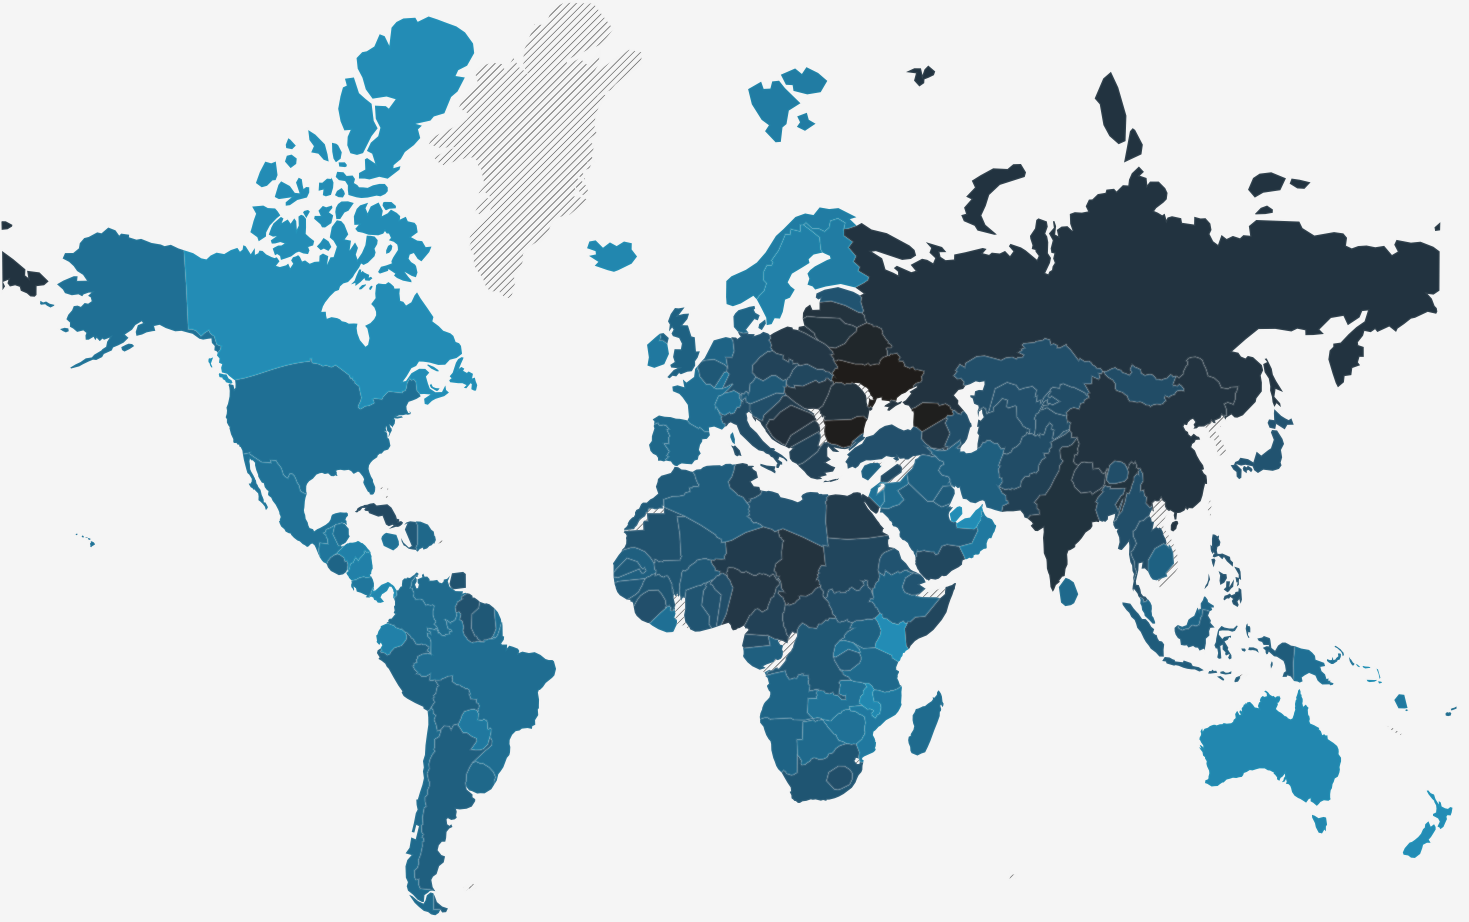
\includegraphics[width=\textwidth]{who.png}
  \caption{\textbf{Reported eaths attributed to air pollution by country (2016)}A cartogram cloropleth showing the number of premature deaths attributed to ambient air pollution per 100,000. The colour bar range is from 9 (light blue) to 170 (navy) people.  Data Source:\citep{whodata}}
  \label{fig:who}
\end{figure}

% \section{composition of the atmosphere}
%
\subsection{Protective barrier - the ozone hole}\label{sec:ozonerole}
Ozone plays a vital role in the stratosphere. This was seen in the 80s where the use of Cloro Floro Carbon (CFC) aerosols resulted in the thinning of the atmospheric ozone \citep{ozonehole}\footnote{Here the chlorine attacks the double bond and `steals' an oxygen atom from the \ch{O3} molecule.}. This resulted in an increase in UV-B radiation, and in consequence skin cancerss, immune supression and disorders of the eye \citep{o3damage}. However since their ban in the Montreal Protocol, the atmospheric hole in ozone has recently recovered to levels similar to its discovery 35 years ago \citep{ozonerepair}.


\subsection{Changing Climate} \label{sec:climatechange}
Over the last 30 years a large body of scientists have established that humans have a warming effect on the planet \citep{IPCC1990Science,IPCC1995Science,IPCC2007Science,IPCC2013Science,ipbes}. Here it has been shown that changes in temperature can lead to the melting of glaciers, rise of sea levels, extreme weather events and the extinction of many species.


\citep{failparis}



\section{Tropospheric Chemistry}

The lowest part of the atmosphere (<18km)\footnote{18km at the tropics, 17km in the mid latitudes and 6km at the poles. } is called the troposphere. This contains ~75\% of the atmospheres mass, and comes from the greek $\tau\rho o \pi o \varsigma$ which means `way' or `turn towards change'. This describes the turbulent mixing that happens due to friction in the lower 2km of the atmosphere (the boundary layer). As the troposphere is the closest part the ground, this where most of the complex chemistry which affects us at the surface happens. This section describes the basic chemical processes which exist in the atmosphere.




\subsection{Ozone Production/Loss}\label{sec:o3prod}
In the troposphere, the mixing ratio of ozone is controlled by the photostationary state relationship (\autoref{eqn:o1}-\ref{eqn:o3}).
Since the concentrations of ozone (20-60 pp\textbf{b}v)\footnote{ppbv: parts per billion volume} are often much higher than that of the nitrogen oxides, NO (1-60 pp\textbf{t}v) and \ce{NO2} (5-70 pp\textbf{t}v), the rapid rate of reaction between \autoref{eqn:o1} does lead to a net change in \ch{o3} concentration \footnote{In urban areas NO concentrations may rise to be be greater than those of \ce{O3} during the night. This leads to a decrease in from \autoref{eqn:o1}} \citep{fundamentals}.



\begin{equation}
  \centering
\ce{NO + O3 ->[k1] NO2 +O2} \label{eqn:o1}
\end{equation}
\begin{equation}
  \centering
 \ce{NO2 + hv ->[J] NO + O }\ \ \ (\lambda < 420nm) \label{eqn:o2}
\end{equation}
 \begin{equation}
   \centering
\ce{O + O2 + M ->[k3] O3 + M}\label{eqn:o3}
\end{equation}

Using \autoref{eqn:o1} and \autoref{eqn:o2} it is possible to describe the change in \ce{NO2} as:

\begin{equation}
  \frac{d[NO_2]}{dt} = k1[NO][O_3] - J[NO_2]
  \label{eqn:ono2}
\end{equation}

If the relative change of \ce{NO2} is small, it can be though of as being in steady state. This means that \autoref{eqn:ono2} can be simplified to producde a relationship between \ch{O3, NO} and \ch{no2} in steady state (\autoref{eqn:oo3}). Here if any two concentrations are known , the third can be calculated.

\begin{equation}
  [O_3] = \frac{J[NO_2]}{k1[NO]}
  \label{eqn:oo3}
\end{equation}

As ozone is a secondary pollutant (made not emitted), and its main reaction produces a null cycle, the production of ozone in the atmosphere requires an increase in nitrogen dioxide concentraions.

% Here it is created and destroyed by the chapman cycle. This is a steady state cycle which...
% However within the troposhere (<15k?) the production and loss of ozone has a direct impact on human life. Polluted environments, such as industrial London,
% SMOG, Clean air act.
% %
%
% NO2 + hv ! NO + O(1D) O(1D)+O2 +M!O3 +M
% ratio of NO and NO2 and the intensity of sunlight (hv), see Fig.1.4.
% [NO2] = k3[O3] (1.4)
% [NO] JN O2
\subsection{The NOx cycle}\label{sec:noxcycle}
Ozone production/loss in the troposphere is directly dependant on the concentration of available Nitrogen Oxides (NOx) (\autoref{sec:o3prod}). These are predominantly emitted by motor verhicles and power stations and can are known to cause respiotory problems in children and asmatics as well as disrupting terrestirial and aquatic ecosystems \citep{eea}. Although NOx may be released naturally, the anthropogenic influence on their emissions was hilighed in early 2020 where the COV-19 corona virus disrupted travel across mainland china, causing a significant drop in anthropogenic emissions - \autoref{fig:chinanox}.

\begin{figure}[H]
    \centering
    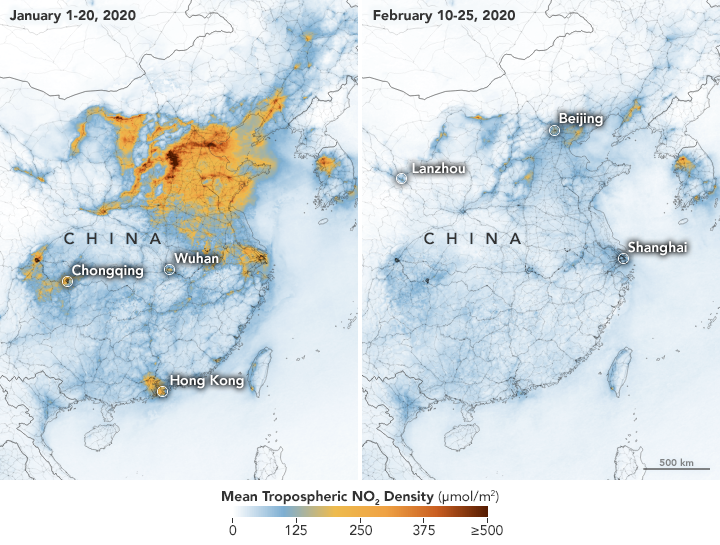
\includegraphics[width=0.7\textwidth]{china_trop_2020056.png}
    \caption{\textbf{Changes in NOx concentrations due to anthropogenic emissions.} A reduction in activity and trasport resutls in a large decrease of Nitrogen dioxide concentrations in the troposphere. Source: \citep{chinanox}}
    \label{fig:chinanox}
\end{figure}

During the day nitrate (\ce{NO3}) radicals can be formed through the reaction with \ch{O3}: \autoref{eqn:ono2} and \autoref{eqn:nno2}, however this is quickly destroyed through rapid photolysis (\autoref{eqn:nno3}) \citep{nitrate}. Photolysis reactions such as \autoref{eqn:nno3} and \autoref{eqn:o2} are no longer possible and th ozone production process shuts down.

\begin{equation}
  \ce{NO2 + O3 ->[k3] NO3 + O2}
  \label{eqn:nno2}
\end{equation}

\begin{equation}
  \ce{NO3 + hv ->[J2] NO2 + O(3P)}
  \label{eqn:nno3}
\end{equation}


 The increased amount of \ce{NO3} can now react with \ce{NO2} to produce dinitric pentoxide (\ce{H2NO5}) and an aqueous nitric acid (\ce{HNO3}) - \autoref{eqn:n2o5} and \autoref{eqn:hno3}. \autoref{eqn:n2o5} is a three body forwards pressure dependant reaction, and a reverse temperature dependant reaction. During the day at the lower troposphere it is warm and this can occur within seconds, however at night or at high altitudes it can take anywhere from hours to months \citep{fundamentals}.


\begin{equation}
  \ce{NO3 + NO2 <=>[M] N2O5 + O}
  \label{eqn:n2o5}
\end{equation}

\begin{equation}
  \ce{N2O5 + H2O ->[k4] 2HNO3}
  \label{eqn:hno3}
\end{equation}



\subsection{HOx Cycle}

The hydroxyl radical (OH) is an important oxidising molecule that initiates the removal of pollutants from the atmosphere. OH is fairly ubiquitous in the atmosphere during the daytime, yet because it is very reactive it typically has an atmospheric lifetime of less than 1 second and an typical ambient concentration of 1 ppt [161]
The reaction of molecules such as VOCs with OH forms more oxidised products, that are more water soluble, and hence it facilitates the removal of pollutants from the atmosphere by wet deposition [188].


%%%%%%%%%%%%%%%%%%%%
% MODEL
%%%%%%%%%%%%%%%%%%%%

\section{Modelling the Earth}
In the previous section the air quality and its detrimental effects on human health was seen to influence polcicy for cities and industry. Koyoto, Islands suing powerstations.
For a policy to be passed there needs to not only evidence of the problem, but a strong suggestion that any proposed changes will have the desired effect. As it is not possible to perform experiments on complex, and often unknown, chemistry at every location on the planet, we are forced to rely on the numerical simulation of the Earth System, and the constituent parts within it.
\subsection{Earth System Models (ESM)}
  ESMs are models capable of predict past or future interactions of the planetary system. They represnt our foremost understanding of the complex interplay between land-surface (geosphere), ocean (hydrosphere), ice (cryosphere) and the air (atmosphere), and act as a surrogate to manual experimentation -  which is just not possible on the global scale.
ESMs can be split into their individial parts. One example of this is the Chemistry section of the Goddard Earth Observing System (an integrated ESM and data assimulation model hosted by NASAs Goddard space flight centre \citep{geoschem}) - GEOS Chem. GEOS-Chem is a global 3D model of atmospheric chemistry which is driven by the meteorology provided by NASA \citep{geos}. Here the earth is split up into cubic sphere cells longitudally and latitudally, as well as vertically (\autoref{fig:gcm})\footnote{This image is not from GEOS-Chem.}. Each one of these cells performs several purtubations of the chemistry within them, before any long-lived species are transported, and the process is repeated. If extracted separately a single one of these cells may be used to explore the sensetivity of different species for a range of input conditions. This is the bases of the atmospheric box model.
\begin{figure}
  \centering
  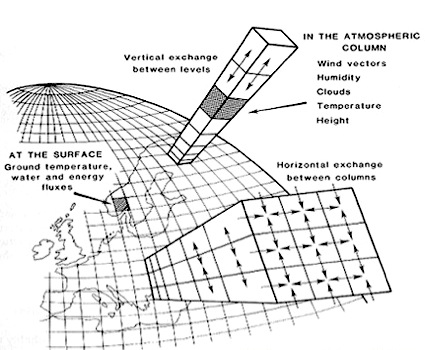
\includegraphics[width=0.6\textwidth]{gcm.jpg}
  \caption{\textbf{A diagram showing the longitudal, lateral and vertical decomposition of a 3D global model.} Source: \citep{gcm}}
  \label{fig:gcm}
\end{figure}
\subsection{The box model.}
In exploring the sensetivities of individual species within a simulation, it is possible to use a zero dimensional box model. This is in essence a single cell within the global structure, constrained in location and height (pressure).
mechanism,
integrator,
etc.

It is then possible to take the many species, their rates or reaction and loss to produce a chemical mechanism detailing their properties in real life.



\subsubsection{Chemical Mechanisms}
Mechanisms are at the heart of every chemistry simulation. They are a mathematical representation of the possible reactions ( and the rates at which these may occur ) for every s
\paragraph{A note on model type, lifetime and mechanism size}
Species such as OH and ... are very short lived and
Ozone for example is long lived and can be transported


\begin{figure}[H]
  \centering
  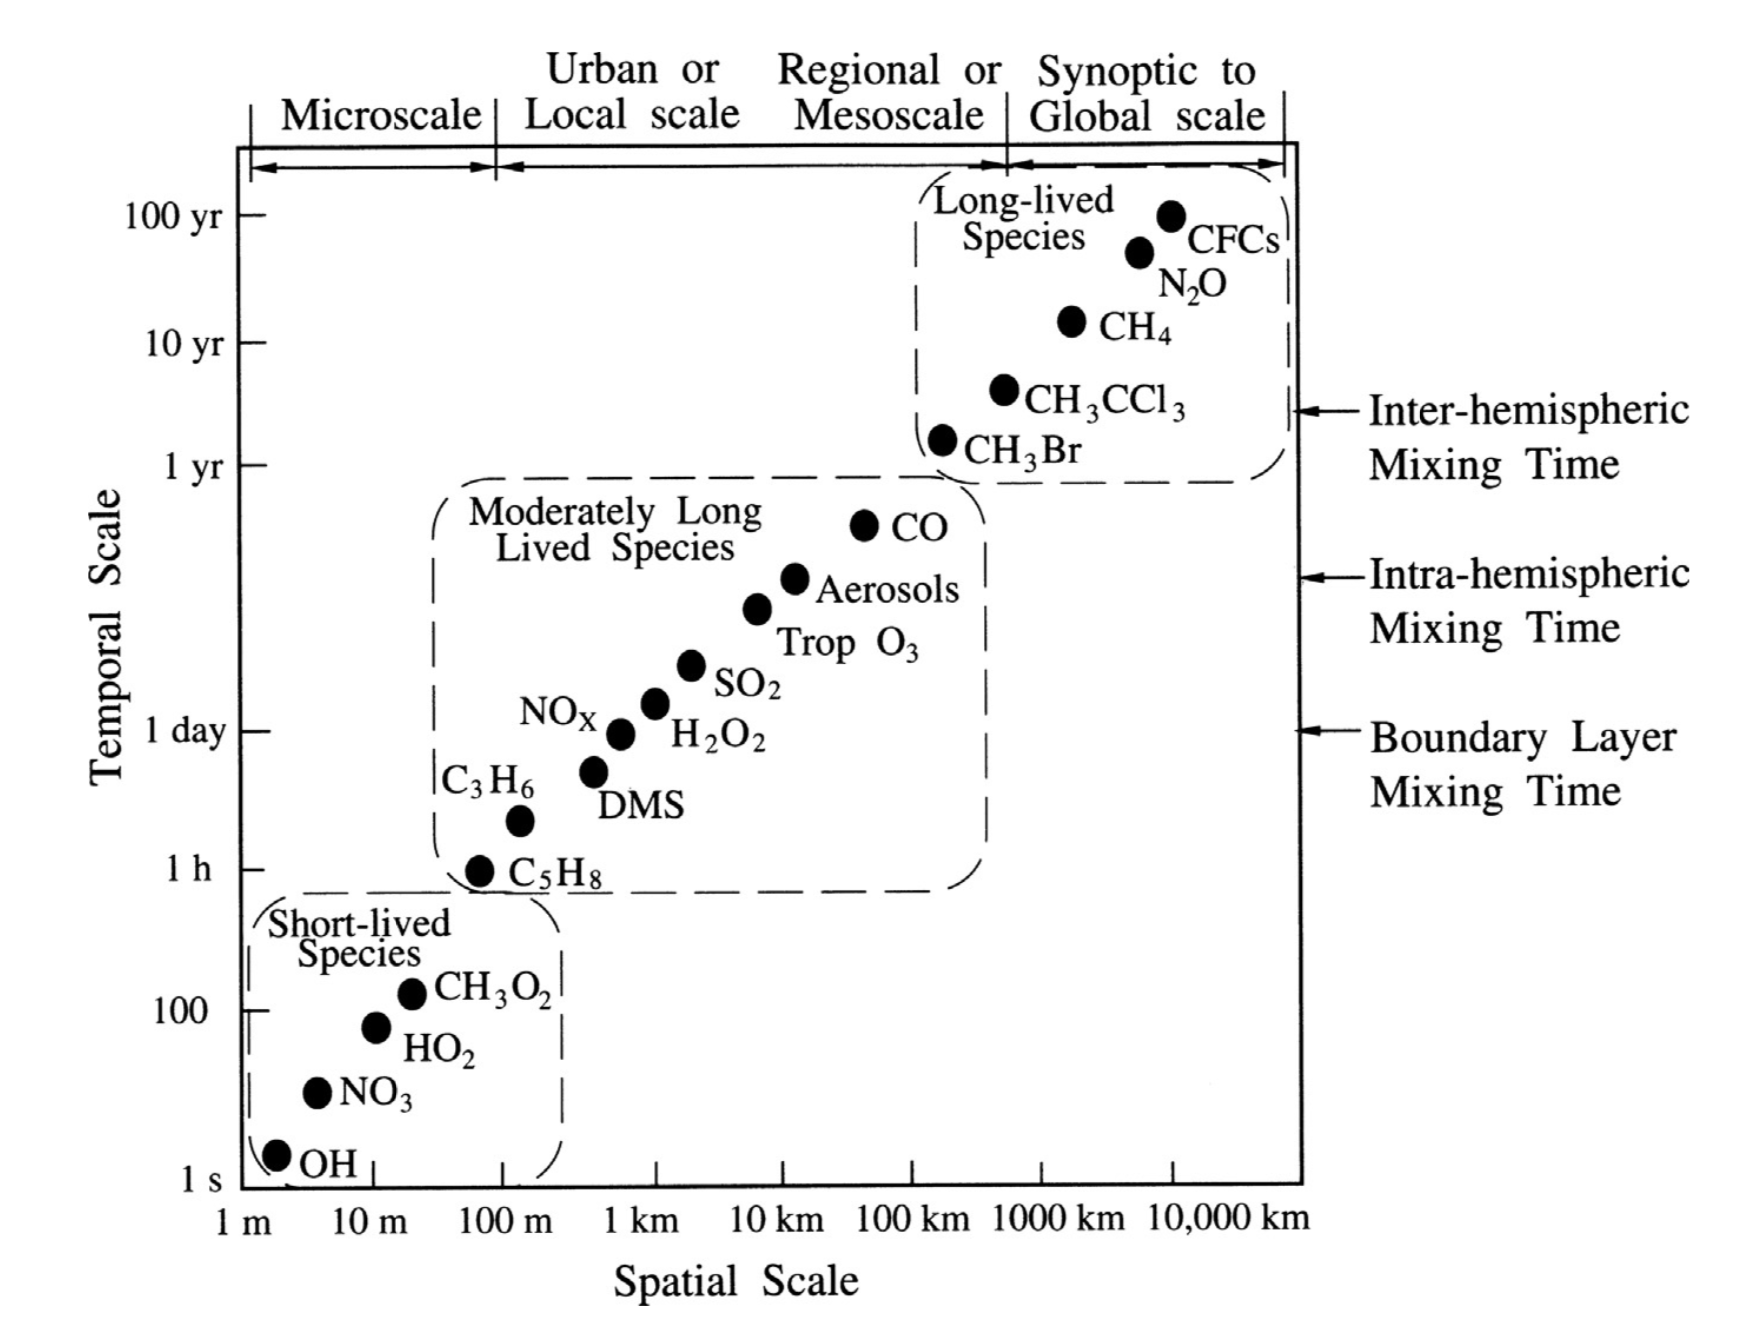
\includegraphics[width=0.7\textwidth]{timescales.png}
  \caption{\textbf{Spatial and temporal scales of variability of atmospheric species.} Source: \citep{transporttime}}
  \label{fig:timescales}
\end{figure}

The atmosphere consists of thousands of species, with tens of thousands of reactions between them.
These models represent real wodlc reactions
In modelling these we can describe their rate of production and loss with respect to the species they react with.
\subsection{Numerical integration}
For example, it is possible to figure out how quickly each species in a reaction is changing if the reaction mechanism (the exact way it happe ns) and some simple data are known. This representation of how quickly the concentrations are changing is the same as a slope, or derivative. Integration allows us to find the actual change over time and not just how quickly the change is happening. Fo r example, given the following reaction,
In a mechanism we are concerned with calculating how quickly a species changes within the chemical system. Taking the reaction of \ch{N2O5} (\autoref{eqn:numerical1}) we can write the rate of change for each species over time (\autoref{eqn:numerical2})\footnote{This is also known as the flux.}. In integrating this equation, we are able to calculate the actual change in concentration (\autoref{eqn:numerical3}) - this is the foundation of atmospheric models.
\begin{equation}
\ce{N2O5 ->	NO2} + \ce{NO3}
\label{eqn:numerical1}
\end{equation}
\begin{equation}
\ce{ d[N2O5]/dt ->	d[NO2]/dt} + \ce{d[NO3]/dt}
\label{eqn:numerical2}
\end{equation}
\begin{equation}
\ce{ \int d[N2O5]/dt ->	\int d[NO2]/dt} + \ce{\int d[NO3]/dt}
\label{eqn:numerical3}
\end{equation}
\subsubsection{Non-Stiff Equations}
Computational systems cannot integrate numbers analytically we rely on a series of computational algorithms. Since integration is the calculation of the area under a curve, the simplest of these
%https://www.ukca.ac.uk/images/b/b1/Solvers_for_web.pdf
\subsubsection{Numerically stiff equations (atmospheric chemistry)}
\autoref{fig:timescales} shows the lifetimes of species can range between x orders of magnitude, similarly the componenets for each reaction (differential equation) evolve on significantly different timescales. This makes the atmospheric chemical mecahnism
\subsection{The model development cycle}
Scientific understanding is the product of many cycles of trial and error, \autoref{fig:devcycle}. In atmospheric chemistry we start with a hypothesis or a question, e.g. will changing X have a negative response on Y. We then construct a theoretical model to represent the chemsistry within. This chemistry is updated to reflect the rates and reactions that have been recorded in laboratory/chamber experiments. This cycle is then repeated until the model and real-world observations produce a comparable result.
\begin{figure}[H]
    \centering
    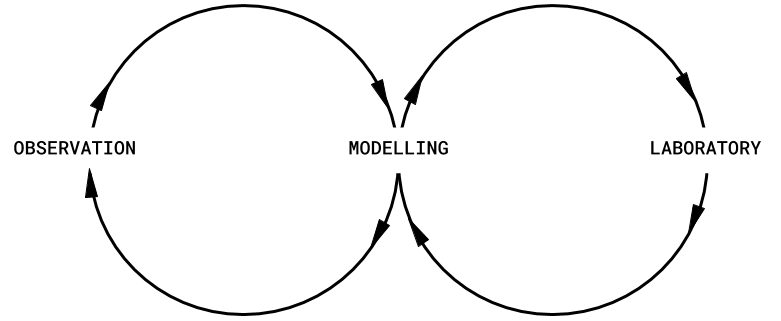
\includegraphics[width=0.6\textwidth]{devcycle.png}
    \caption{\textbf{The scientific development cycle.}This shows the iterative nature between modelling, observation and laboratory experimentation}
    \label{fig:devcycle}
\end{figure}

ESM
 A series of box models.
 \subsection{The Dynamically Simple Model of Atmospheric Chemical Complexity}


 % Early simulations, such
 %
 % as those run on ENIAC2, were capable of success-
 % ful 24 hour weather prediction. Unfortunately, al-
 % though a great feat, the delay in simulation time re-
 % sulted in a computation that only just kept up with
 %
 % real-life events [Lynch, 2008]. in 1995 a general circu-
 % lation model of the atmosphere was created by Phillips
 %
 % [Phillips, 1956]. It was soon discovered that this was
 % insu
 % cient to represent the Earth, and a general Global
 % Climate Model (GCM) was formed from the union
 % of atmospheric, oceanic, cryospheric and land-surface
 %
 % models [NIPCC, 2010]. The outcome of this was a pro-
 % gram capable of simulating accurate short-term weather
 %
 % predictions, which can allow an insight into the con-
 % tributing factors of climate change.
 %
 %
 % \subsubsection{Common Problems with Earth prediction}
 % There are several problems that an earth simulation model can face, most of which can be attributed to computational efficiency. An example of this is seen with the
 %
 % MET - DAY TO SIMULATE
 %
 % Other problems with meteorlogy that are encountered rest on resolution. Too fine a scale and the model can take forever to run. simplfy, lose local effect and islands.
 %
 % Finally the tuning of models can result in overfitting due to a limited understanding or dataset. Here a model may be tweked to ..
 %
 % Numerical stiff chemical complexity.
 %
 %


 %%%%%%%%%%%%%%%%%%%%
 % Thesis
 %%%%%%%%%%%%%%%%%%%%

\section{Thesis Layout}
This thesis will explore a series of methods for describing and understaning the complex chemistry which may exist as part of an atmospheric chemistry mechanism. The mechanism used is a near-explicit representation of our foremost understanding of how gas phase chemistry in the troposphere reacts - the Master Chemical Mechanism, \citep{mcm}.
We begin by exploring the use of visualisation to convey complex scientific data (\autoref{ch1}). Next we apply this to the representation of species in a mechanism, and the relationships between them. To do this it is found that the node-link style graph format is the most beneficial, the use of which is then explored further (\autoref{ch2}).
However in doing so, large complex network are shown to reach the limits of human cognition and visual representation. To overcome this a series of mathematic metrics are used to leverage our understanding of the species in a chemical network using graph theory (\autoref{ch3}). The use of computation to aid in graph analysis is further extended when graph clustering methods are applied as a method to group similar species within a chemical network (\autoref{ch4}). Finally in a bid towards the use of graph neural networks (see future work, \autoref{sec:futurework}), a range of different chemical representations for machine learning are explored using a number of dimensionality reduction algorithms (\autoref{ch5}).
